\documentclass[xcolor=dvipsnames]{beamer}

\usepackage[utf8]{inputenc}
\usepackage[english]{babel}
\usepackage[T1]{fontenc}
\usepackage{xcolor}

\usepackage{amsmath}
\usepackage{amssymb}
\usepackage{amsfonts}
\usepackage{times}
\usepackage{autobreak}
\usepackage{relsize}
\usepackage{enumerate}
\usepackage{booktabs}
\usepackage{color}
\usepackage{graphicx}
\usepackage{epstopdf}
\usepackage{float}
\usepackage{placeins}
\usepackage[caption=false]{subfig}
\usepackage{hyperref}
\usepackage[toc,page]{appendix}

\graphicspath{./image/Image}

%%%%%%%%%%%%%%%%%%%%%%%%%%%%%%%%%%%%%%%%
\usetheme{Berlin}
%\usecolortheme[named=Blue]{structure}

\definecolor{lightgray}{gray}{0.95}
\definecolor{myellow}{RGB}{255,255,0}
\setbeamercolor{background canvas}{bg=lightgray}
\setbeamercolor{section in head/foot}{fg=white}
\setbeamercolor{title}{fg=myellow}
\setbeamercolor{frametitle}{fg=myellow}
\setbeamercolor{block title}{fg=white}

\usefonttheme{structurebold}

\useinnertheme{circles}
\useinnertheme{rounded}

\makeatletter
\setbeamertemplate{headline}{
  \begin{beamercolorbox}[ht=2.25ex,dp=2.85ex]{section in head/foot}
    \insertnavigation{\paperwidth}
  \end{beamercolorbox}
}

\setbeamertemplate{frametitle}{
  \nointerlineskip
  \begin{beamercolorbox}[sep=0.4ex,wd=\paperwidth]{frametitle}
    \vskip-0.5ex
    \strut\insertframetitle\strut
  \end{beamercolorbox}
}
\makeatother

\usepackage{appendixnumberbeamer}

%%%%%%%%%%%%%%%%%%%%%%%%%%%%%%%%%%%%%%%%
\title[Parameter Estimation of Gravitational Wave Data]
{Parameter Estimation of Gravitational Wave Data}

\author[Chia-Jui Chou]
{\Large{Chia-Jui Chou}\\
\small{National Yang Ming Chiao Tung University, Taiwan}}

\institute[2025/04/24]
{2023/04/24}

\date[2023/04/24]
{}

%%%%%%%%%%%%%%%%%%%%%%%%%%%%%%%%%%%%%%%%
\begin{document}

\begin{frame}
  \titlepage
\end{frame}

%\begin{frame}{Outline} \label{outline}
%  \tableofcontents
%\end{frame}

\setcounter{equation}{0}
\renewcommand{\theequation}{\arabic{section}.\arabic{equation}}

%%%%%%%%%%%%%%%%%%%%%%%%%%%%%%%%%%%%%%%%
\section[PE and Bayesian Inference]{Parameter Estimation and Bayesian Inference}

\begin{frame}[t]{Detection of Gravitational Waves: Matched Filtering}
  If we have some knowledge of $h(t)$, by multiplying $s(t)$ and $h(t)$:
  \begin{equation*}
    \frac{1}{T} \int_0^T s(t) h(t) dt = \frac{1}{T} \int_0^T h^2(t) dt + \frac{1}{T} \int_0^T n(t) h(t) dt,
  \end{equation*}
  where
  \begin{equation*}
    \frac{1}{T} = \int_0^T h^2(t) dt \sim h_0^2, \quad \frac{1}{T} \int_0^T n(t) h(t) dt \sim \left( \frac{\tau_0}{T} \right)^{1/2} n_0 h_0.
  \end{equation*}

  Optimal Signal-to-Noise Ratio:
  \begin{equation*}
    \left( \frac{S}{N} \right)^2 = 4 \int_0^\infty \frac{|\tilde{h}(f)|^2}{S_n(f)} df, \quad \langle |\tilde{n}(f)|^2 \rangle = \frac{1}{2} S_n(f) T.
  \end{equation*}
\end{frame}

\begin{frame}[t]{Parameter Estimation of Gravitational Waves Signal}
  \begin{itemize}
    \item There are models describing gravitational wave form the coalescence binary compact objects: IMRPhenom, SEOBNR, SpinTaylor, IMRSpinPrecEOB...
    \item From the strain data of an event, we estimate the most probable model and the parameters.
    \item Intrinsic Parameters: $m_1, m_2, a_1, a_2, \theta_1, \theta_2, \delta \phi, \phi_{jl}$.
    \item Extrinsic Parameters: $ra, dec, \theta_{jn}, \psi, d_L, \phi_c, t_c$.
  \end{itemize}
\end{frame}

\begin{frame}[t]{Bayes' Theorem}
  \begin{block}{Bayes' Theorem}
    \begin{equation*}
      p(\theta_i | d, H) = \frac{p(d | \theta_i, H) p(\theta_i | H)}{p(d | H)}.
    \end{equation*}
  \end{block}
  \begin{itemize}
    \item $H$: model,
    \item $\theta_i$: parameters for the model $H$,
    \item $d$: observed data,
    \item $p(\theta_i | H)$: prior,
    \item $p(d | \theta_i, H)$: likelihood,
    \item $p(\theta_i | d, H)$: posterior,
    \item $p(d | H)$: evidence.
  \end{itemize}
\end{frame}

\begin{frame}[t]{Bayes' Theorem}
  \begin{block}{Marginalization}
    \begin{equation*}
      p(\theta_1 | d, H) = \int_{\theta_2^\text{min}}^{\theta_2^\text{max}} \cdots \int_{\theta_N^\text{min}}^{\theta_N^\text{max}} p(\theta_1, \cdots, \theta_N | d, H) d\theta_2 \cdots d\theta_N.
    \end{equation*}
  \end{block}
  \begin{block}{Evidence}
    \begin{equation*}
      p(d | H) = \int_{\theta_1^\text{min}}^{\theta_1^\text{max}} \cdots \int_{\theta_N^\text{min}}^{\theta_N^\text{max}} p(\theta_1, \cdots, \theta_N | d, H) d\theta_1 \cdots d\theta_N.
    \end{equation*}
  \end{block}
\end{frame}

\begin{frame}[t]{Evaluating Posterior}
  \begin{block}{Bayes' Theorem}
    \begin{equation*}
      p(\theta_i | d, H) = \frac{p(d | \theta_i, H) p(\theta_i | H)}{p(d | H)} = \frac{L(\theta_i) \cdot \pi(\theta_i)}{Z}.
    \end{equation*}
  \end{block}
  \begin{itemize}
    \item We don't know the normalization constant $Z$.
    \item Use Markov Chain Monte Carlo algorithms to generate samples from $L(\theta_i) \cdot \pi(\theta_i)$ in the parameter space.
  \end{itemize}
  \begin{equation*}
    L(\theta_i) = \mathcal{N} \exp \left\{ -\frac{1}{2} \Big( s - h(\theta_i) | s - h(\theta_i) \Big) \right\},
  \end{equation*}
  where
  \begin{equation*}
    (A|B) = 4 \text{Re} \int_0^\infty \tilde{A}^\ast(f) [S_n^{-1}(f)] \tilde{B}(f) df.
  \end{equation*}
\end{frame}

\begin{frame}[t]{Markov Chain Monte Carlo Algorithm}
  Generate a Markov Chain:
  \begin{equation*}
    \left\{ \theta_i^{(0)} \rightarrow \theta_i^{(1)} \rightarrow \theta_i^{(2)} \rightarrow \cdots \rightarrow \theta_i^{(N)} \right\},
  \end{equation*}
  The steps are stochastic and determined by the probabilities $T(\theta_i, \theta_i^{\prime})$ associated with the trasition $\theta_i \rightarrow \theta_i^{\prime}$.
  \begin{itemize}
    \item $T(\theta_i, \theta_i^{\prime}) \ge 0.$
    \item The posterior is an invariant distribution of the chain: $p(\theta_i^{\prime} | d, H) = \int p(\theta_i | d, H) T(\theta_i, \theta_i^{\prime}) d\theta_i.$
    \item Detailed Balance: $p(\theta_i | d, H) T(\theta_i, \theta_i^{\prime}) = p(\theta_i^{\prime} | d, H) T(\theta_i^{\prime}, \theta_i)$
    \item Ergodicity:
    \begin{itemize}
      \item $\exists n ~ \text{such that} ~ T^n(\theta_i, \theta_i^{\prime}) > 0 ~ \text{for all} \quad \theta_i, \theta_i^{\prime},$
      \item $\exists \theta_i ~ \text{such that} ~ T(\theta_i, \theta_i) > 0.$
    \end{itemize}
  \end{itemize}
\end{frame}

\begin{frame}[t]{Markov Chain Monte Carlo Algorithm}
  \begin{center}
  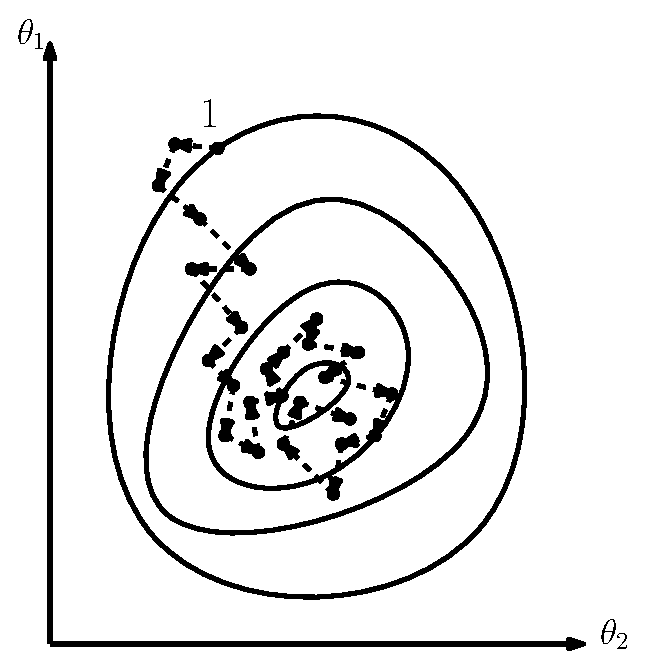
\includegraphics[height=0.8\textheight]{./image/mcmc.eps}
\end{center}
\end{frame}

\begin{frame}[t]{Metropolis-Hasting Sampling}
  \begin{enumerate}
    \item Starting at a random $\theta_i^{(0)}$ in the parameter space.
    \item An update proposal $\theta_i^{\prime}$ of $\theta_i^{(k)}$ is generated by sampling form a known proposal distribution $\tilde{p}(\theta_i^{\prime})$ (e.g. Gaussian distribution centered at $\theta_i^{(k)}$).
    \item Acceptance: $A(\theta_i^{(k)}, \theta_i^{\prime}) = \min{\left( 1, \frac{p(\theta_i^{\prime})}{p(\theta_i^{(k)})} \frac{\tilde{p}(\theta_i^{(k)})}{\tilde{p}(\theta_i^{\prime})} \right)}$.
    \item If $A(\theta_i^{(k)}, \theta_i^{\prime}) \ge 1$ (accepted): record $\theta_i^{(k+1)} = \theta_i^{\prime}$, \\
    else:
    \begin{itemize}
      \item $\theta_i^{(k+1)} = \theta_i^{\prime}$ with the probability: $\frac{p(\theta_i^{\prime})}{p(\theta_i^{(k)})} \frac{\tilde{p}(\theta_i^{(k)})}{\tilde{p}(\theta_i^{\prime})}$.
      \item $\theta_i^{(k+1)} = \theta_i^{(k)}$ with the probability: $1 - \frac{p(\theta_i^{\prime})}{p(\theta_i^{(k)})} \frac{\tilde{p}(\theta_i^{(k)})}{\tilde{p}(\theta_i^{\prime})}$.
    \end{itemize}
  \end{enumerate}
\end{frame}

\begin{frame}[t]{Metropolis-Hasting Sampling}
  \begin{itemize}
    \item Now the Markov chain we get: $\left\{ \theta_i^{(0)} \rightarrow \cdots \rightarrow \theta_i^{(N)} \right\}$ can be considered as a correction of the proposal distribution $\tilde{p}(\theta_i)$ to the posterior distribution $p(\theta_i | d, H)$.
    \item Now Drawing the histogram plot of $\left\{ \theta_i^{(0)}, \cdots, \theta_i^{(N)} \right\}$, we can see the distribution proportional to the posterior and find out the most probable parameters.
  \end{itemize}
\end{frame}

\begin{frame}[t]{Nested Sampling}
  \begin{itemize}
    \item MCMC methods: Generates samples proportional to the the posterior.
    \item Nested Sampling: Simultaneously estimates the evidence and the posterior.
  \end{itemize}
  Pros of Nested Sampling:
  \begin{itemize}
    \item well-defined stopping criteria for terminating sampling,
    \item generating a sequence of independent samples,
    \item flexibility to sample from complex, multi-modal distributions,
    \item the ability to derive how statistical and sampling uncertainties impact results from a single run,
    \item being trivially parallelizable.
  \end{itemize}
\end{frame}

\begin{frame}[t]{Nested Sampling}
  \begin{block}{Prior Mass}
    \begin{equation*}
      X(\lambda) = \int_{\theta: L(\theta) > \lambda} \pi(\theta) d\theta.
    \end{equation*}
  \end{block}
  \begin{block}{Evidence}
    \begin{equation*}
      Z = \int_0^1 L(X) dX, \quad \text{where} \quad L(X(\lambda)) = \lambda.
    \end{equation*}
  \end{block}
\end{frame}

\begin{frame}[t]{Nested Sampling}
  \begin{center}
    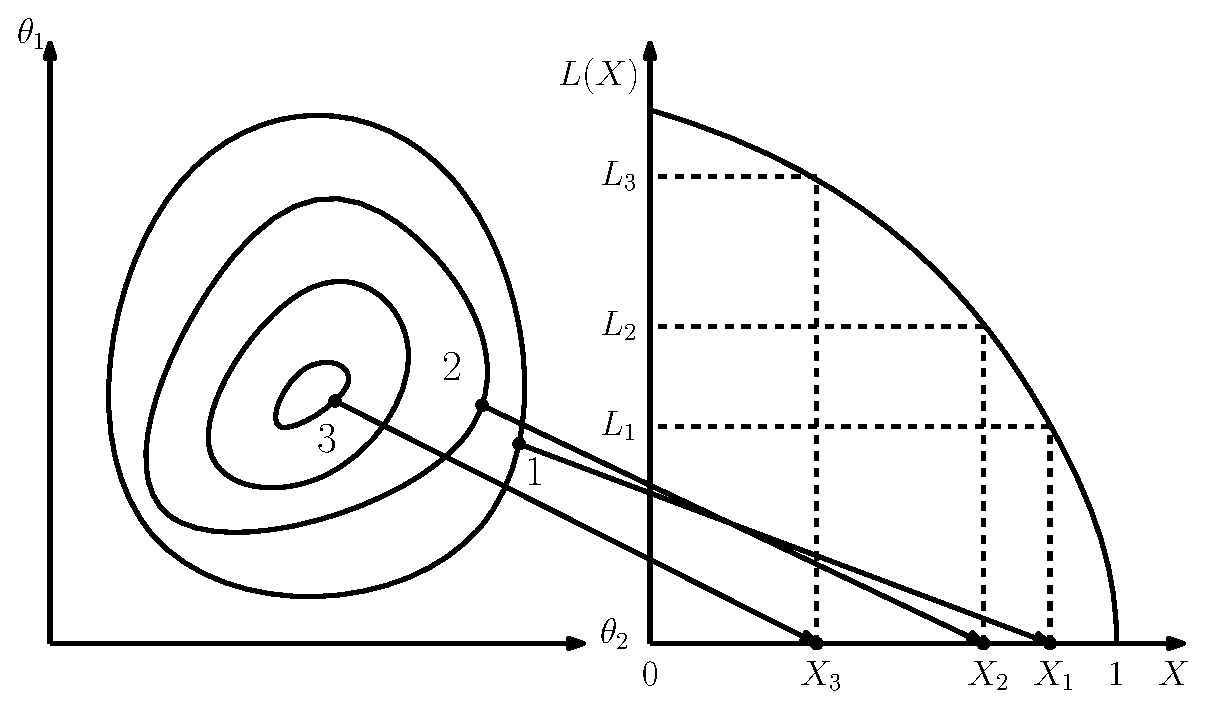
\includegraphics[height=0.75\textheight]{./image/prior_mass.eps}
  \end{center}
\end{frame}

\begin{frame}[t]{Nested Sampling}
  \begin{center}
    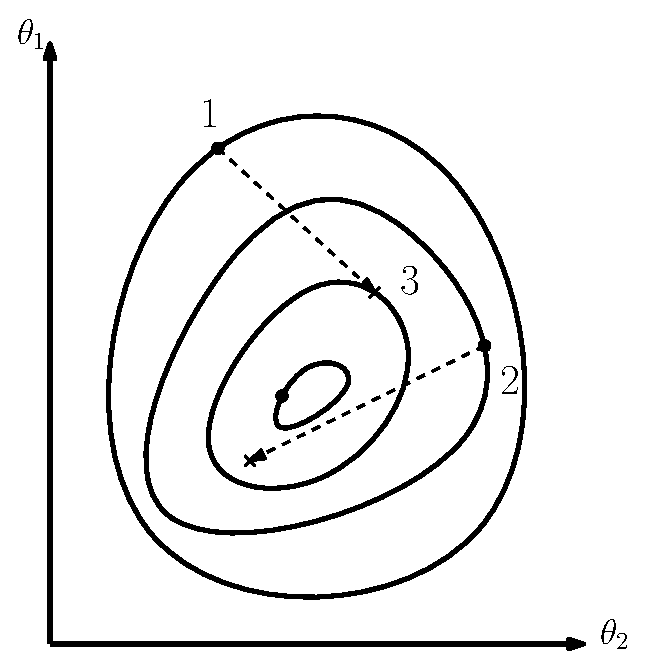
\includegraphics[height=0.8\textheight]{./image/nested_sampling.eps}
  \end{center}
\end{frame}

\begin{frame}[t]{Nested Sampling}
  \begin{enumerate}
    \item Sample N live points $\{ \theta^{(1)} \cdots \theta^{(N)} \}$ from prior $\pi(\theta)$.
    \item While not termination condition:
      \begin{enumerate}
        \item record live point $(i)$ with the lowest $L_i$ as $L_k$,
        \item assign $X_k = t_k X_{k-1}$ where $t_k$ from $P(t_k) = N t_k^{N-1}$,
        \item replace point $(i)$ with sample from $\pi(\theta)$ subject to $L_i > L_k$.
      \end{enumerate}
    \item Estimate evidence $Z$ by integrating $\{ L_k, X_k \}$.
  \end{enumerate}
\end{frame}

%%%%%%%%%%%%%%%%%%%%%%%%%%%%%%%%%%%%%%%%
\section[Bilby]{Bilby: Bayesian inference library}

\begin{frame}[c]{Using Bilby for Parameter Estimation}
  \begin{enumerate}
    \item Get strain data,
    \item Estimate Power Spectral Density,
    \item Determine Waveform model,
    \item Set the prior distributions of the estimated parameters,
    \item Set likelihood,
    \item Set the sampler,
    \item Run the sampler!
    \item Plot the results.
  \end{enumerate}
\end{frame}

\begin{frame}[c]{}
  \begin{center}
    
\includegraphics[scale=0.5]{image/Thankyou.png}
  \end{center}
\end{frame}

%%%%%%%%%%%%%%%%%%%%%%%%%%%%%%%%%%%%%%%%
\appendix
\section{Appendices}

\iffalse
%%%%%%%%%%%%%%%%%%%%%%%%%%%%%%%%%%%%%%%%
\section[Introduction to GW]{Introduction to Gravitational Wave}

\begin{frame}[t]{General Relativity: Einstein Equation}
  \begin{block}{Einstein Equation}
    \begin{equation*}
      R_{\mu\nu} - \frac{R}{2} g_{\mu\nu} = \frac{8\pi G}{c^4} T_{\mu\nu},
    \end{equation*}
  \end{block}
  \begin{itemize}
    \item $g_{\mu\nu}$: metric tensor,
    \item $R_{\mu\nu}$: Ricci tensor,
    \item $R = g^{\mu\nu} R_{\mu\nu}$: Ricci scalar,
    \item $T_{\mu\nu}$: stress-energy tensor.
  \end{itemize}
  \begin{block}{Measure of interval in spacetime}
    \begin{equation*}
      ds^2 = g_{\mu\nu} dx^\mu dx^\nu.
    \end{equation*}
  \end{block}
\end{frame}

\begin{frame}[t]{General Relativity: Linearized Theory}
  \begin{block}{Perturbation of metric tensor}
    \begin{equation*}
      g_{\mu\nu} = \eta_{\mu\nu} + h_{\mu\nu}, \quad |h_{\mu\nu}| \ll 1.
    \end{equation*}
  \end{block}
  \begin{block}{Linearized Einstein Equation}
    \begin{equation*}
      \Box \bar{h}_{\mu\nu} + \eta_{\mu\nu} \partial^\rho \partial^\sigma \bar{h}_{\rho\sigma} - \partial^\rho \partial_\nu \bar{h}_{\mu\rho} - \partial^\sigma \partial_\mu \bar{h}_{\nu\rho} = -\frac{16\pi G}{c^4} T_{\mu\nu}.
    \end{equation*}
  \end{block}
  \begin{itemize}
    \item $h = \eta^{\mu\nu} h_{\mu\nu}$,
    \item $\bar{h}_{\mu\nu} = h_{\mu\nu} - \frac{1}{2} \eta_{\mu\nu} h$.
  \end{itemize}
\end{frame}

\begin{frame}[t]{Harmonic Gauge and Transverse-Traceless Gauge}
  \begin{block}{Harmonic Gauge}
    \begin{equation*}
      \partial^\nu \bar{h}_{\mu\nu} = 0.
    \end{equation*}
  \end{block}
  \begin{block}{Linearized Einstein Equation}
    \begin{equation*}
      \Box \bar{h}_{\mu\nu} = 0,
    \end{equation*}
  \end{block}
  $T_{\mu\nu} = 0$ if we observe the GW far away from the source.
  \begin{block}{Transverse-Traceless Gauge}
    \begin{equation*}
      h^{0\mu}, \quad h^i_i = 0, \partial^j h_{ij} = 0,
    \end{equation*}
  \end{block}
  which can only be chosen away from the source.
\end{frame}

\begin{frame}[t]{Solution of the Gravitational Wave}
  We can choose the propagation direction along $\hat{z}$, with the wave vector:
  \begin{equation*}
    k^\mu = (\omega/c, \mathbf{k}),
  \end{equation*}
  and the solution of GW:
  \begin{equation*}
    h^{\text{TT}}_{\mu\nu} (t, z) =
    \begin{pmatrix}
      0 & 0 & 0 & 0 \\
      0 & h_{+} & h_{\times} & 0 \\
      0 & h_{\times} & -h_{+} & 0 \\
      0 & 0 & 0 & 0
    \end{pmatrix}
    \cos \left[ \omega(t - z/c) \right].
  \end{equation*}
  The we have the perturbed metric tensor:
  \begin{align*}
    ds^2 = & -c^2 dt^2 + dz^2 + \left\{ 1 + h_{+}\cos[\omega(t - z/c)] \right\} dx^2 \\
    & - \left\{ 1 + h_{+}\cos[\omega(t - z/c)] \right\} dy^2 + 2h_{\times}\cos[\omega(t - z/c)] dxdy.
  \end{align*}
\end{frame}

\begin{frame}[t]{Gravitational Wave Interacting with Test Masses}
  \begin{center}
    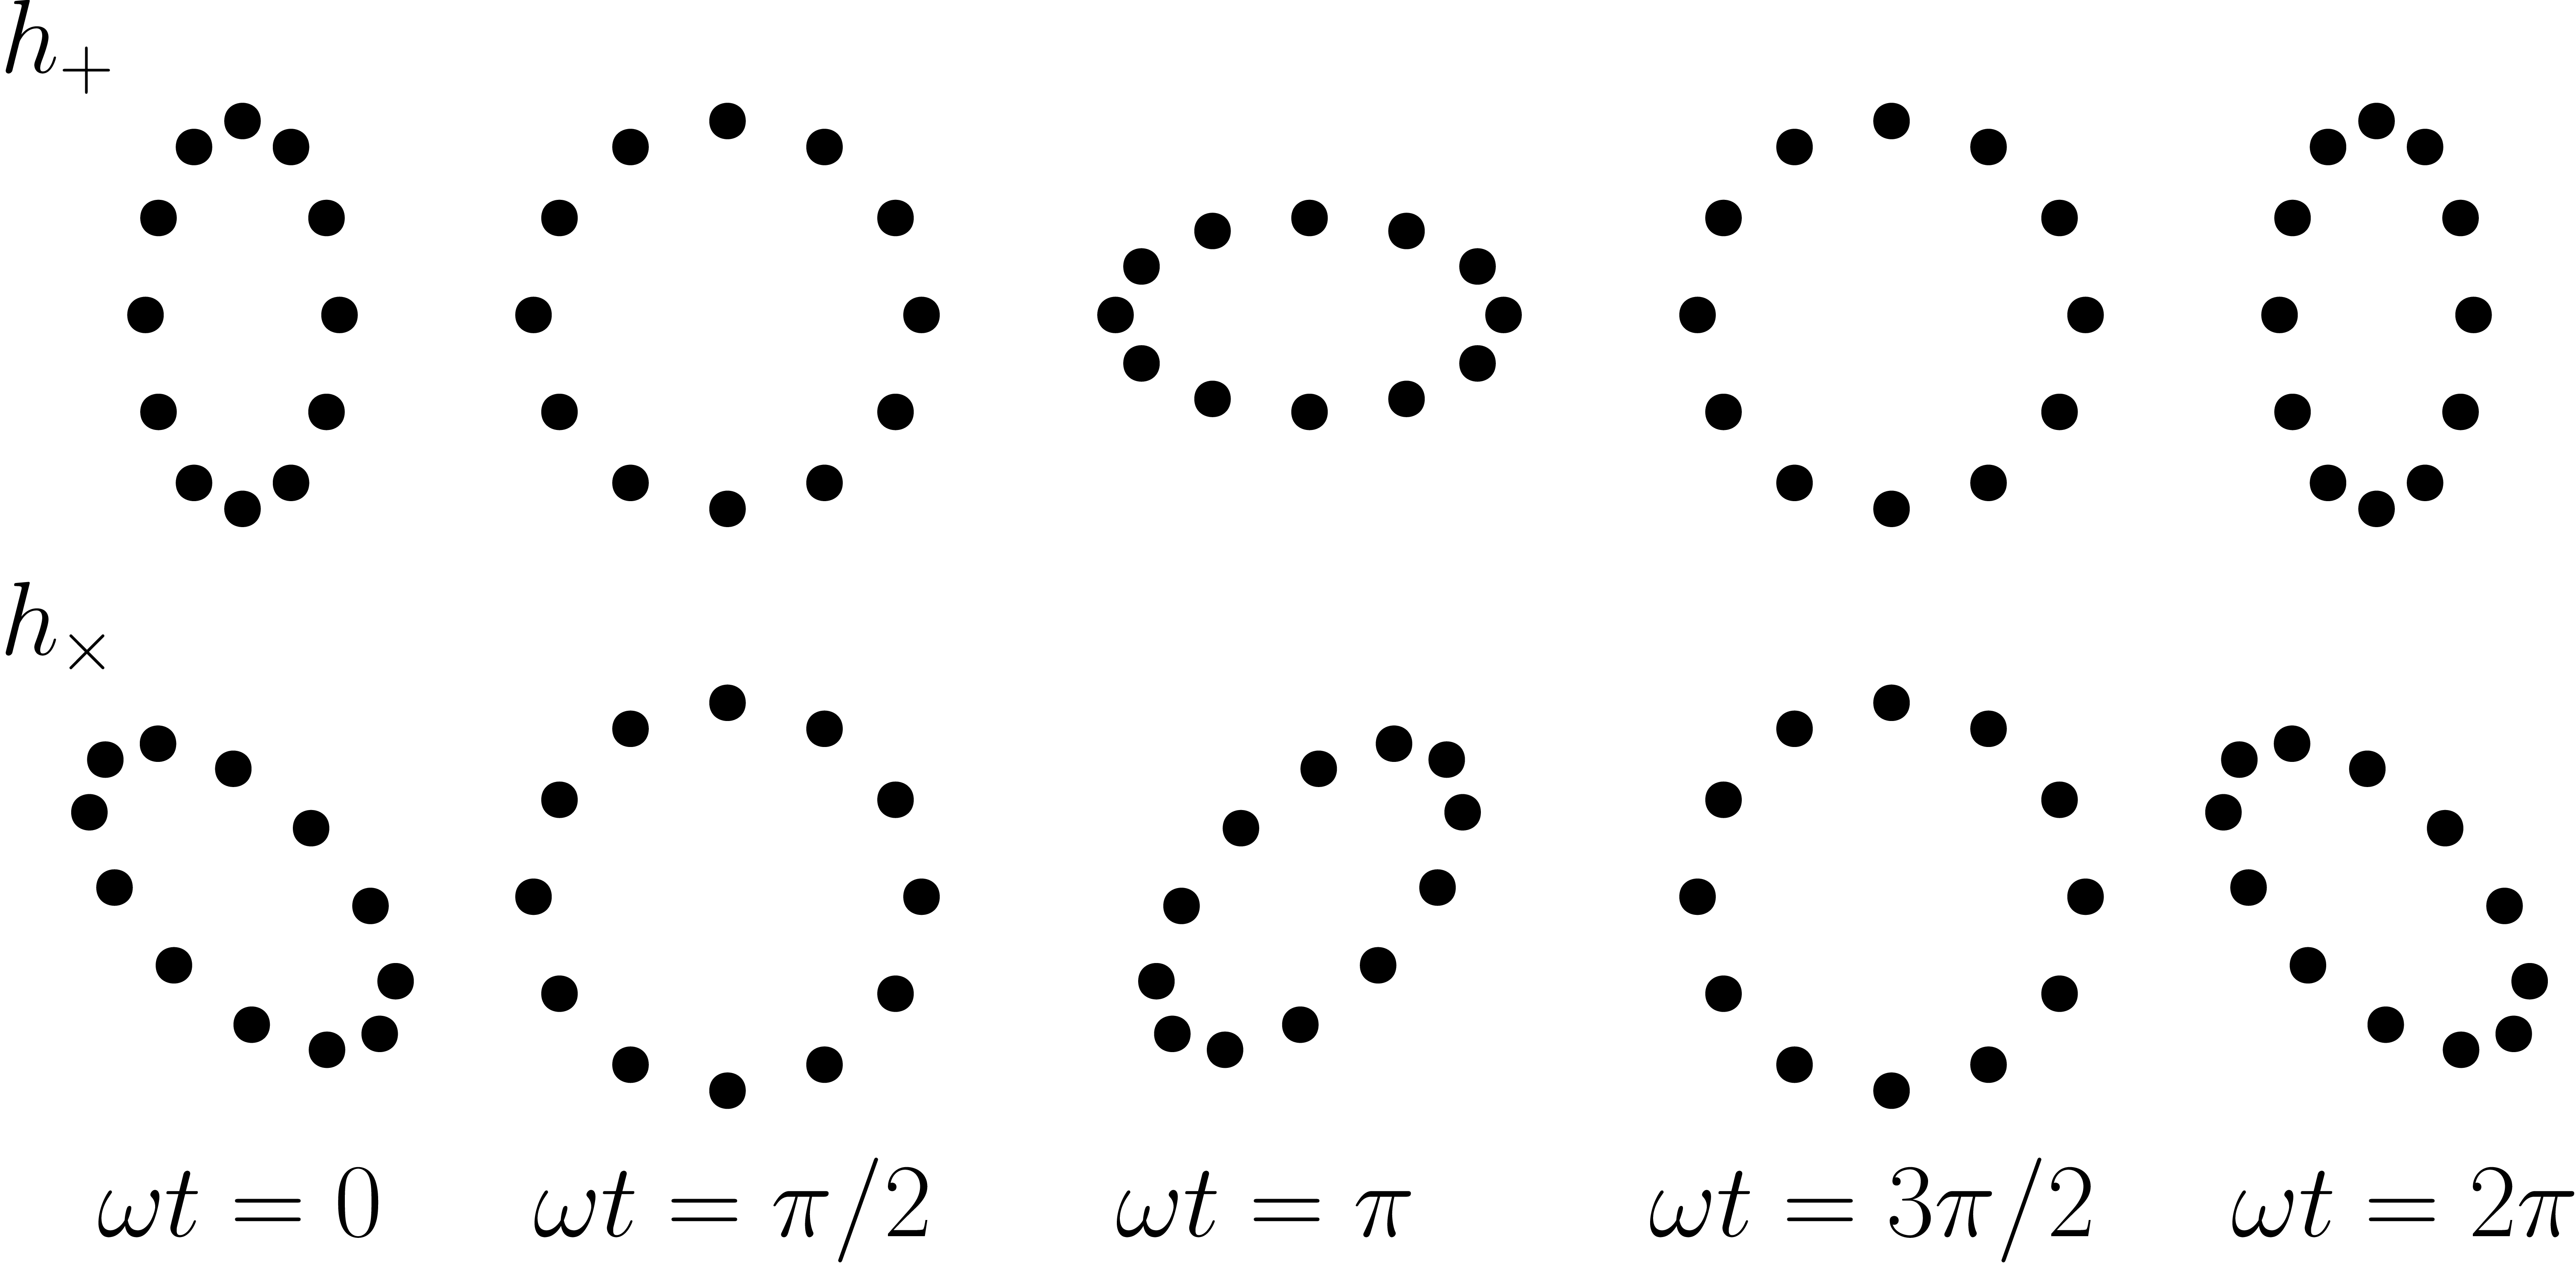
\includegraphics[width=\textwidth]{image/test-mass.eps}
  \end{center}
\end{frame}

\begin{frame}[t]{Sources of Gravitational Waves}
  \begin{itemize}
    \item Compact Binary Coalescence:
    \begin{itemize}
      \item Black Hole-Black Hole Merger,
      \item Neutron Star-Neutron Star Merger,
      \item Black Hole-Neutron Star Merger.
    \end{itemize}
    \item Continuous Wave Sources:
    \begin{itemize}
      \item Spping Neutron Star,
      \item Pulsar.
    \end{itemize}
    \item Burst Sources:
    \begin{itemize}
      \item Supernovae,
      \item Gamma-ray Burst.
    \end{itemize}
    \item Stochastic Background:
    \begin{itemize}
      \item Primordial background,
      \item Astrophysical background.
    \end{itemize}
  \end{itemize}
\end{frame}

\begin{frame}[t]{Gravitational Wave Detector}
  \begin{center}
    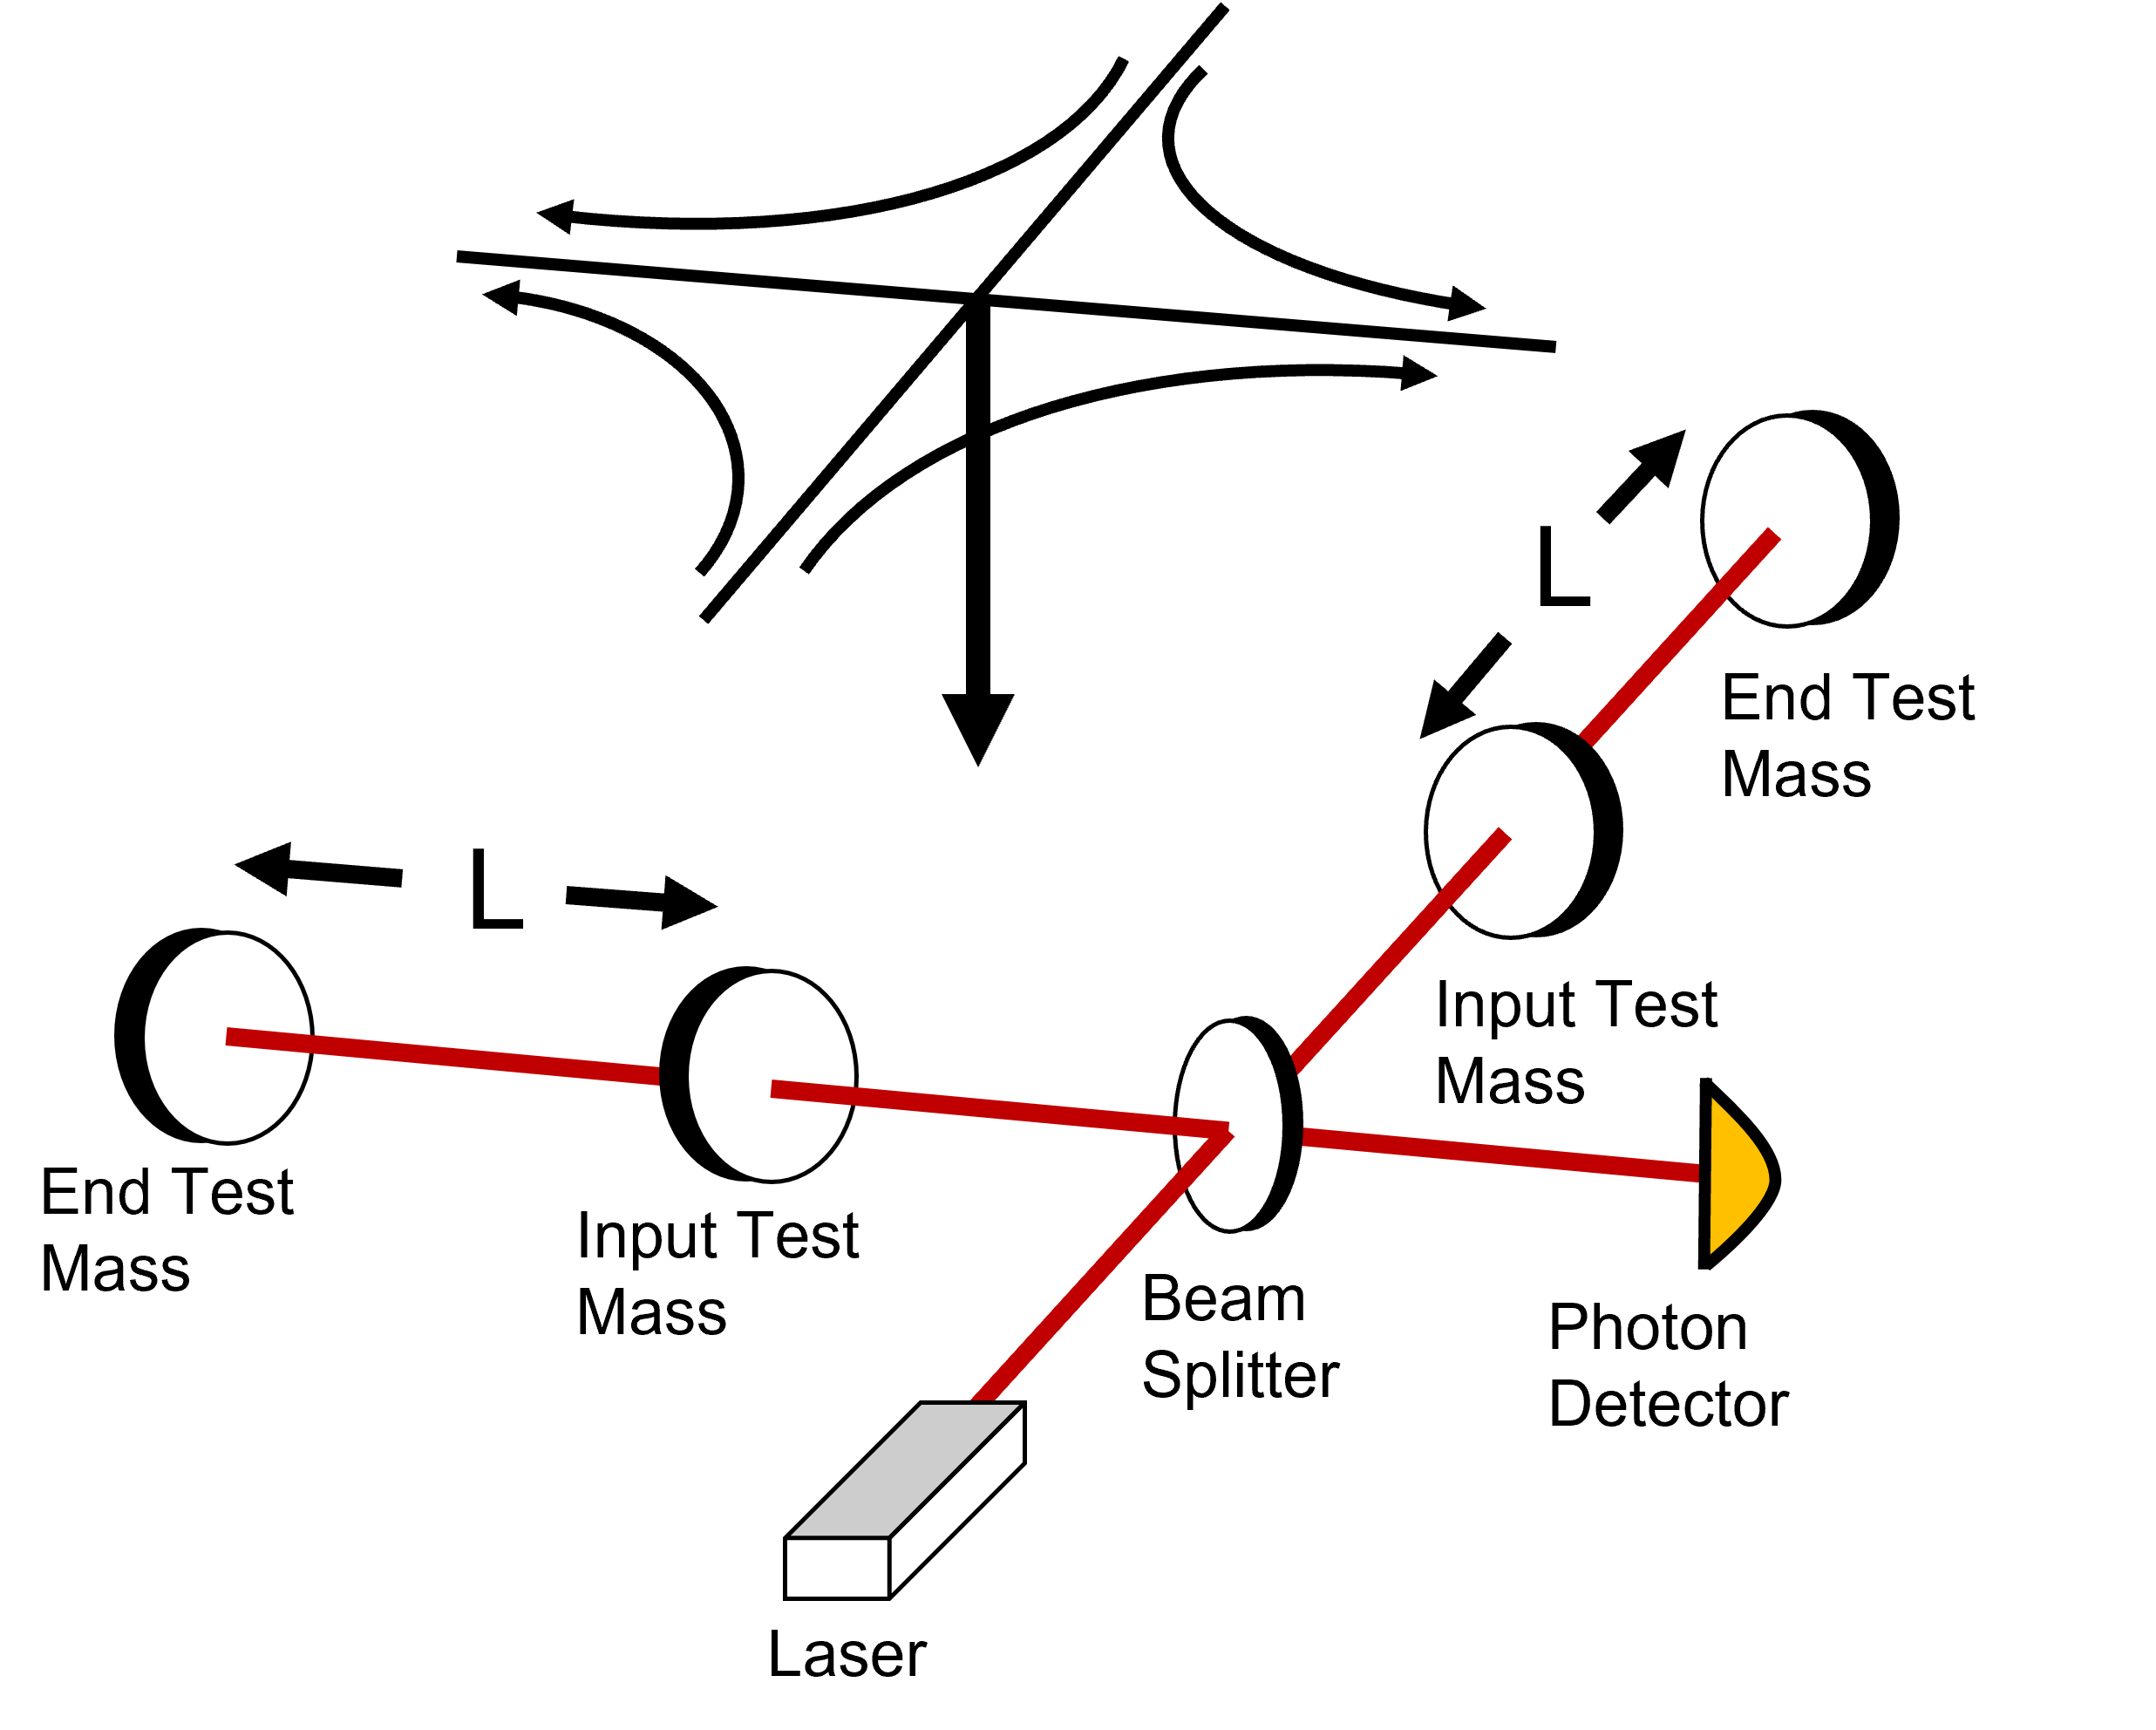
\includegraphics[height=0.8\textheight]{./image/GW-detector.png}
  \end{center}
\end{frame}

\begin{frame}[t]{Gravitational Wave Detector}
  \begin{columns}
    \begin{column}{0.5\textwidth}
      \begin{center}
        \includegraphics[width=0.9\textwidth]{./image/GWeffect2.png}
      \end{center}
    \end{column}
    \begin{column}{0.5\textwidth}
      \begin{center}
        \includegraphics[width=0.9\textwidth]{./image/GWeffect1.png}
      \end{center}
    \end{column}
  \end{columns}
\end{frame}

%%%%%%%%%%%%%%%%%%%%%%%%%%%%%%%%%%%%%%%%
\section[Offline Deepclean]{Offline Cleaning on O3GK Data}

\begin{frame}[t]{Offline Cleaning on O3GK Data}
	We pick the intervals from O3GK data to test on Deepclean:
	\begin{itemize}
		\item 1271260000 \char`\~ 1271263000
	\end{itemize}
	\begin{center}
		\includegraphics[scale=0.5]{./image/60Hz_DQ_1271250000-1271300000.png}
	\end{center}
\end{frame}

\begin{frame}[t]{Subtracting 60Hz AC Power Noise}
	\begin{itemize}
  {\footnotesize{
    \item PEM channels: \\
      K1:PEM-SENSOR\_RACK\_OMC1\_DSUB(1 \char`\~ 3)\_OUT\_DQ, \\
      K1:PEM-VOLT\_PSL\_TABLE\_GND\_OUT\_DQ, \\
      K1:PEM-VOLT\_PSL\_BOOTH\_FLOAT\_OUT\_DQ, \\
      K1:PEM-VOLT\_AS\_TABLE\_GND\_OUT\_DQ, \\
      K1:PEM-VOLT\_OMC\_CHAMBER\_GND\_OUT\_DQ, \\
      K1:PEM-VOLT\_REFL\_TABLE\_GND\_OUT\_DQ
    \item Strain channels: K1:DAC-STRAIN\_C20
    \item Sampling rate: 4096Hz
    \item Bandpass filter: 55Hz \char`\~ 65Hz
    \item Batch size: 32
    \item Epoches: 20
    \item Loss function: $J_{asd}$
    \item Training time: from {\color{blue}1271260000 \char`\~ 1271261000}
  }}
  \end{itemize}
\end{frame}

\begin{frame}[t]{Test: Clean from 1271261000 for 2000s}
	\begin{center}
		\includegraphics[height=0.2\textwidth]{./image/AC/raw_strain-1271261000-2000.png}
		\includegraphics[height=0.2\textwidth]{./image/AC/predicted_strain-1271261000-2000.png}
		\includegraphics[height=0.2\textwidth]{./image/AC/cleaned_strain-1271261000-2000.png}
	\end{center}
\end{frame}

\begin{frame}[t]{Test: Clean from 1271261000 for 2000s}
  Amplitude Spectral Density of the strains:
  \begin{center}
    \includegraphics[width=1.0\textwidth]{./image/AC/asd_60.png}
  \end{center}
\end{frame}

\begin{frame}[t]{Test: Clean from 1271261000 for 2000s}
  Coherence between strains and witness channels:
  \begin{center}
    \includegraphics[width=\textwidth]{image/AC/coherence_K1PEM-SENSOR_RACK_OMC1_DSUB1_OUT_DQ.png}
  \end{center}
\end{frame}

\begin{frame}[t]{Test: Clean from 1271261000 for 2000s}
  Coherence between strains and witness channels:
  \begin{center}
    \includegraphics[width=\textwidth]{image/AC/coherence_K1PEM-SENSOR_RACK_OMC1_DSUB2_OUT_DQ.png}
  \end{center}
\end{frame}

\begin{frame}[t]{Test: Clean from 1271261000 for 2000s}
  Coherence between strains and witness channels:
  \begin{center}
    \includegraphics[width=\textwidth]{image/AC/coherence_K1PEM-SENSOR_RACK_OMC1_DSUB3_OUT_DQ.png}
  \end{center}
\end{frame}

\begin{frame}[t]{Test: Clean from 1271261000 for 2000s}
  Coherence between strains and witness channels:
  \begin{center}
    \includegraphics[width=\textwidth]{image/AC/coherence_K1PEM-VOLT_AS_TABLE_GND_OUT_DQ.png}
  \end{center}
\end{frame}

\begin{frame}[t]{Test: Clean from 1271261000 for 2000s}
  Coherence between strains and witness channels:
  \begin{center}
    \includegraphics[width=\textwidth]{image/AC/coherence_K1PEM-VOLT_OMC_CHAMBER_GND_OUT_DQ.png}
  \end{center}
\end{frame}

\begin{frame}[t]{Test: Clean from 1271261000 for 2000s}
  Coherence between strains and witness channels:
  \begin{center}
    \includegraphics[width=\textwidth]{image/AC/coherence_K1PEM-VOLT_PSL_BOOTH_FLOAT_OUT_DQ.png}
  \end{center}
\end{frame}

\begin{frame}[t]{Test: Clean from 1271261000 for 2000s}
  Coherence between strains and witness channels:
  \begin{center}
    \includegraphics[width=\textwidth]{image/AC/coherence_K1PEM-VOLT_PSL_TABLE_GND_OUT_DQ.png}
  \end{center}
\end{frame}

\begin{frame}[t]{Test: Clean from 1271261000 for 2000s}
  Coherence between strains and witness channels:
  \begin{center}
    \includegraphics[width=\textwidth]{image/AC/coherence_K1PEM-VOLT_REFL_TABLE_GND_OUT_DQ.png}
  \end{center}
\end{frame}
\fi

\end{document}